% \begin{columns}
%     \begin{column}{0.5\textwidth}
%     
%     \end{column}
% \end{columns}
% \begin{columns}
%     \begin{column}{0.5\textwidth}
%     
%     \end{column}
% \end{columns}

%   \begin{wrapfigure}[8]{r}{0.4\textwidth}
%     \begin{minipage}{\dimexpr\linewidth-2\fboxrule-2\fboxsep}
%     {\tiny
%     \begin{lstlisting}
%        @ @ @   @       @     @ @     @ @ @     @ @ @ @  @ @ @    @ @ @
%       @        @ @   @ @   @     @   @     @   @        @     @  @     @
%       @        @   @   @  @       @  @      @  @        @     @  @     @
%         @ @    @       @  @       @  @      @  @ @ @    @ @ @    @ @ @
%             @  @       @  @       @  @      @  @        @   @    @
%             @  @       @   @     @   @     @   @        @    @   @
%        @ @ @   @       @     @ @     @ @ @     @ @ @ @  @     @  @
% 
%       \  \  /   / /    \   \  /   \  /    /     /        @ @ @   @ @ @
%        \ _\/   /_/      \   \/     \/    /_____/        @     @  @     @
%            \__/          \  /      _\___/                     @  @      @
%                \____      \/      /                          @   @      @
%                     \_____/______/                         @     @      @
%                                  \                       @       @     @
%                                   \____________________ @ @ @ @  @ @ @
%     \end{lstlisting}
%     }
%     \end{minipage}
%   \end{wrapfigure}
%----------------------------------------------------------------------------------------
%   Summary
%----------------------------------------------------------------------------------------



\begin{alertblock}{Summary}
    {\large
    \begin{itemize}
        \item Parameters of surface runoff model were derived for each soil texture (past work)
        \item Newly the parameters were derived with optimization on extended set of data
        \item Sensitivity analysis were performed 
        \item Uncertainly of parameters were assessed with Monte Carlo simulations 
        \item New open source model provider is presented 
    %       \item
    %       \item
    \end{itemize}
    }
%     In the past parameters of the phy\-sically-based, distributed, event runoff/erosion SMODERP2D Model were inferred for each soil textural class. This approach were performed to simplify practitioners life since the parameters were ready to use if one have the soil texture of the area of interest. In order to assess variability of each parameter within and across textural classes the model were optimized to laboratory artificial rainfall experiments at 4 different textural classes. 
%     Results shows that ...
\end{alertblock}\vspace{0.9cm}



%----------------------------------------------------------------------------------------
%   INTRODUCTION
%----------------------------------------------------------------------------------------


\mojesekce{Material and Methods}
\subsection{Model structure}
\begin{block}{Model structure}
    Based on a balance equation 
    $$
        \frac{Storage}{\Delta t} = \nonumber  
        Inflow - Outflow
    $$
    is inferred bucket model with kinematic wave approach for momentum 
    $$
%       \begin{split}
        \frac{\partial h_{i}}{\partial t} =  es_{i} + \sum_j^n q_{j} - inf_{i} - q_{i} - ret_i
    $$
    where $h$ is water level [$L$], $es$ is effective precipitation [$L.T^{-1}$], $inf$ is infiltration [$L.T^{-1}$], $ret$ surface retention [$L$], and $q$ is the Manning-Strickler formula
    \begin{equation}
      q = Xi^Yh^b. 
      \label{eq:manning}
    \end{equation}

    {\bf Parameters $X$, $Y$, and $b$ were inferred for each soil textural class.} Variability of those parameters within and among textural classes is assessed in this poster. Infiltration is solved with Phillip's infiltration equation:
    \begin{equation}
      inf = 1/2St^{-1/2} + Ks.
      \label{eq:Phillips}
    \end{equation}
    {\bf Saturated hydraulic conductivity $Ks$ [$L.T^{-1}$] and sorptivity $S$ [$L.T^{-1/2}$] were fitted with measured data.}
\end{block}



\subsection{Current  parameter values}
\begin{block}{Current  parameter values}\vspace{-1cm}
\begin{columns}
    \begin{column}{0.25\textwidth}
        \justifying
        Actual parameter values were inferred based on rainfall simulations and shallow water flow experiments~\cite{kavka}
    \end{column}
    \begin{column}{0.75\textwidth}
        \begin{table}[]
            \small
            \caption{Current parameter set for soil textural classes}
            \begin{tabular}{lllll|lllll}
            \hline
            \hline
            Textural class & ID  & $b$    & $X$    & $Y$     & Textural class  & ID   & $b$    & $X$    & $Y$  \\
            \hline
            sand           & SS  & 1.82 & 8.81 & 0.366 & sandy clay loam & SCL  & 1.7  & 10.7 & 0.603 \\
            loamy sand     & LS  & 1.82 & 8.81 & 0.366 & clay loam       & CL   & 1.7  & 10.7 & 0.603 \\
            sandy loam     & SL  & 1.79 & 9.2  & 0.462 & silty clay loam & SICL & 1.7  & 10.7 & 0.603 \\
            loam           & LL  & 1.74 & 10.1 & 0.561 & sandy clay      & SC   & 1.67 & 11.3 & 0.636 \\
            silt loam      & SIL & 1.74 & 10.1 & 0.561 & silty clay      & SIC  & 1.67 & 11.3 & 0.636 \\
            silt           & SI  & 1.74 & 10.1 & 0.561 & clay            & CC   & 1.67 & 11.3 & 0.636 \\
            \hline
            \hline
            \end{tabular}
        \end{table}
    \end{column}
\end{columns}
    
\end{block}

\subsection{Soil classes and ARE overview}
\begin{block}{Soil classes and ARE overview}
    \begin{itemize}
        \item 266 experiments with artificial rainfall were performed 
        \item Various slopes and rainfall intensities were tested for each location.
    \end{itemize}\vspace{-1cm}
% 
    \begin{columns}
        \begin{column}{0.4\textwidth}
            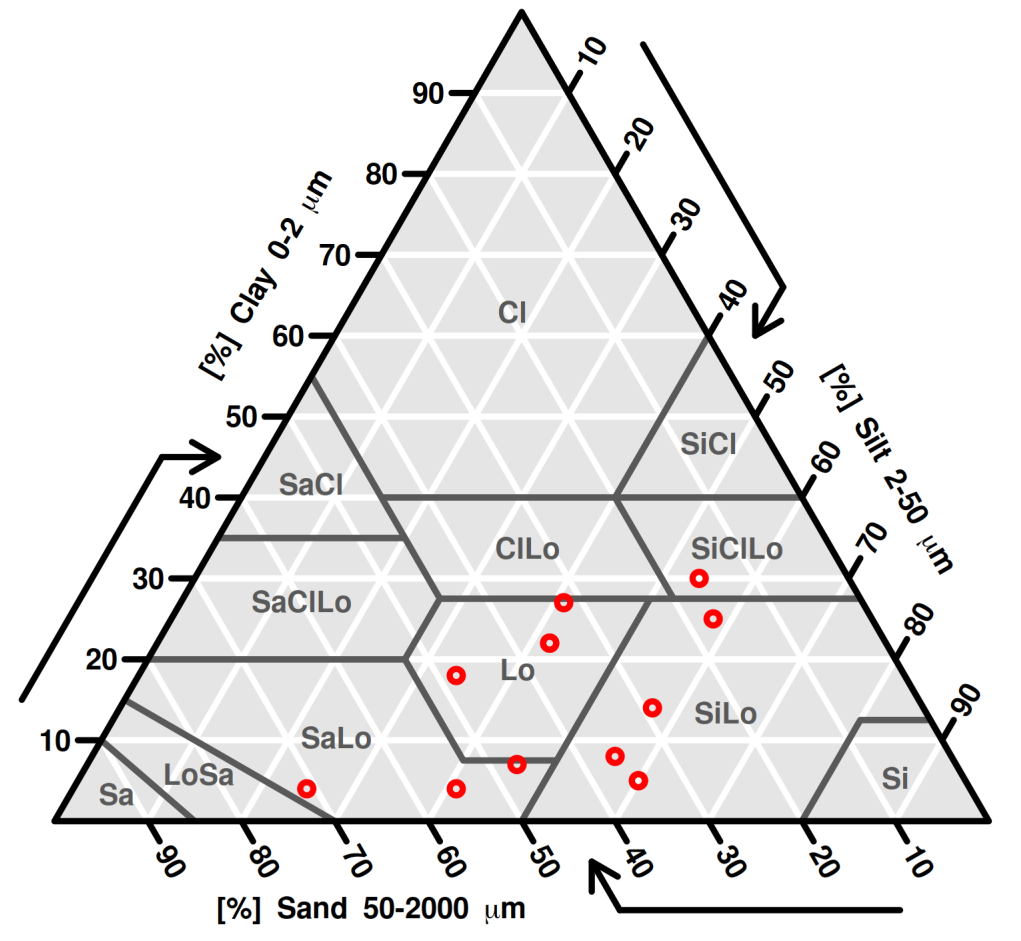
\includegraphics[width=.95\textwidth]{obr/soil_triangle.png}
        \end{column}
        \begin{column}{0.6\textwidth}
            {\small 
            \begin{table}[]
            \caption{Overview of artificial rainfall experimets}
                \begin{tabular}{lcccccc}
                \hline
                \hline
                location      & year    & no. of            & \multicolumn{3}{c}{soil texture {[}\%{]}}  & soil class      \\
                            &         & exper.       & clay  & silt  & sand &  \\
                \hline
                Horoměřice    & 2002    & 25                & 25             & 58            & 17            & silty loam      \\
                Třebsín I     & 2004    & 22                & 5              & 60            & 35            & silty loam      \\
                Neustupov     & 2006    & 14                & 4              & 41            & 55            & sandy loam      \\
                Klapý         & 2007    & 25                & 30             & 54            & 16            & silty clay loam \\
                Třebsín II    & 2008    & 28                & 5              & 60            & 35            & silty loam      \\
                Třebešice I   & 2009    & 27                & 4              & 25            & 71            & sandy loam      \\
                Třebešice II  & 2010    & 36                & 7              & 46            & 47            & sandy loam      \\
                Nučice        & 2011    & 35                & 14             & 57            & 29            & silty loam      \\
                Všetaty I     & 2012    & 24                & 22             & 42            & 36            & loam            \\
                Všetaty II    & 2013    & 17                & 22             & 42            & 36            & loam            \\
                Třebešice III & 2014    & 22                & 8              & 56            & 36            & silty loam      \\
                Nové Strašecí & 2015    & 20                & 27             & 41            & 32            & loam            \\
                Řisuty        & 2017    & 21                & 18             & 34            & 48            & loam           \\
                \hline
                \hline
                \end{tabular}
            \end{table}
            }
        \end{column}
    \end{columns}
\end{block}



        
